%%%%%%%%%%%%%%%%%%%%%%%%%%%%%%%%%%%%%%%%%%%%%%%%%%%%%%%%%%%%%%%%%%%%%%%%%%%%%%%%
%%%%%%%%%%%%%%%%%%%%%%%%%%%%%%%%%%%%%%%%%%%%%%%%%%%%%%%%%%%%%%%%%%%%%%%%%%%%%%%%
%%%%%%%%%%%%%%%%%%%%%%%%%%%%%%%%%%%%%%%%%%%%%%%%%%%%%%%%%%%%%%%%%%%%%%%%%%%%%%%%
Este capítulo descreve com detalhes o ambiente de desenvolvimento que foi realizado neste projeto.

\section{Ambiente proposto}%

	O desenvolvimento do ambiente foi realizado para a plataforma web. Consiste em três partes principais:
	
	\begin{itemize}
		\item Editor de texto
		\item Montador
		\item Simulador
	\end{itemize}

	Toda a parte de interação com o usuário utiliza as tecnologias web: \textit{javascript}, para ter uma interface dinâmica, utilizando a biblioteca \textit{jQuery}. Para a estruturação utilizou-se a linguagem de marcação \textit{HTML}, e a folha de estilos \textit{CSS} para formatação do layout.

	Apesar de ter sido desenvolvido para rodar na web, os componentes "Montador" e "Simulador", podem ser utilizados separados, por exemplo em linha de comando. Basta ter instalado um interpretador \textit{Python 3.x}


\section{Arquitetura de software}

	Como na maioria das aplicações web, utilizamos o modelo Cliente-Servidor. Neste modelo, o usuário é um cliente, que faz requisições ao servidor. 

	Neste projeto o usuário faz requisição da página inicial, onde ele pode escrever seu código, então a partir disso ele irá enviar este código para o servidor, requisitando a montagem, e então receberá a saída do montador, ou a mensagem apropriada no caso de erros.

	Com o código montado, pode se salvar em arquivos os dados da montagem em diferentes formatos, binário, hexadecimal ou em formato \textit{MIF ("Memory Initialization File")}, utilizado para inicializar memórias em FPGA's da Altera. Esses dados podem ser enviados novamente para o servidor em uma nova requisição de simulação, e então o servidor irá responder os resultados do programa, qual o estado de memória final, valores dos registradores, e se houver, mensagens de saída.



	- modelo cliente servidor
	- api

\section{Interface web}

	A interface web foi feita com as tecnologias padrões da web, HTML, CSS e Javascript. E faz parte do frontend da aplicação, onde o usuário irá interagir com a ferramenta. 

	Para a parte dinâmica do site foi utilizada a biblioteca jQuery, facilitando o desenvolvimento de funcionaliades no front-end principalmente na manipulação de elementos da tela. 

	Para o layout foi utilizado o framework Materialize CSS, com sua utilização perdemos menos tempo em detalhes de layout, e podemos focar mais nas funcionalidades.


	\begin{figure}
	  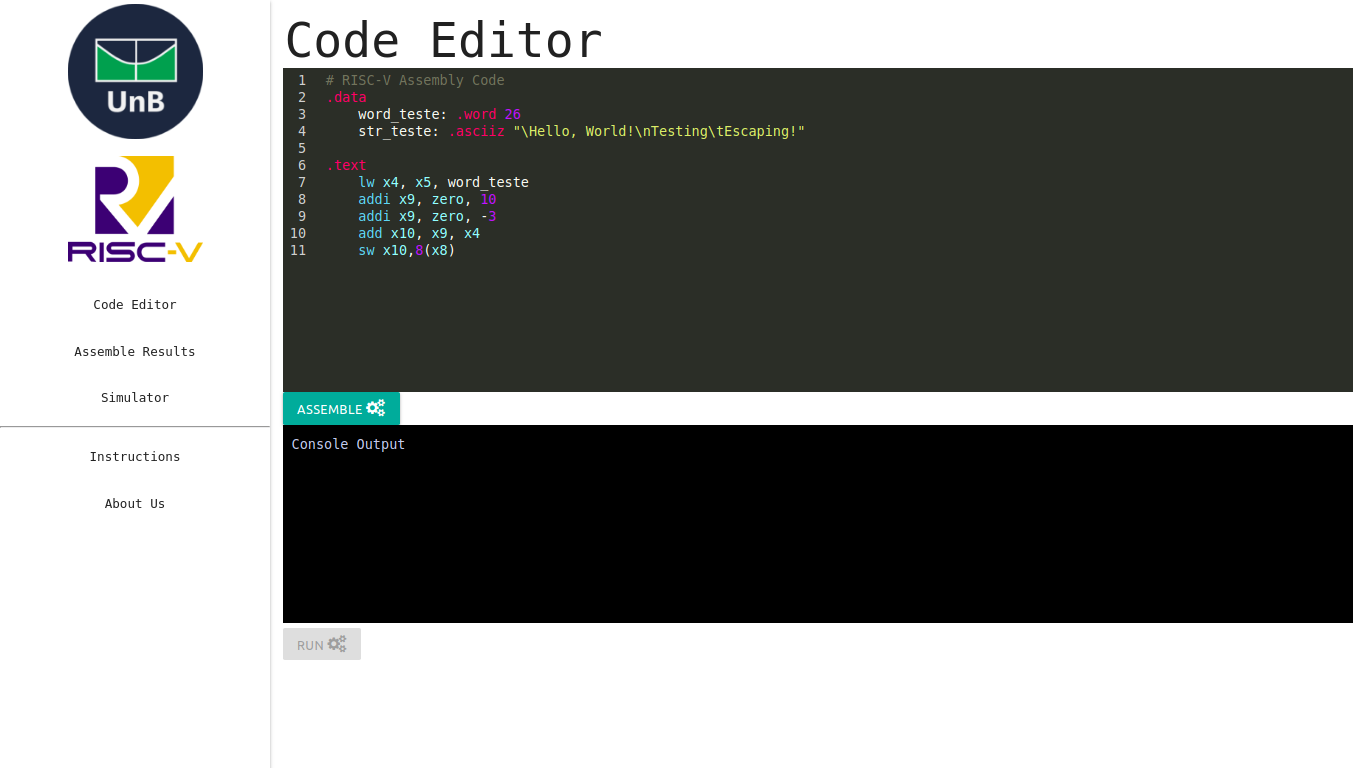
\includegraphics[width=\linewidth]{img/code_editor.png}
	  \caption{Página inicial, mostra o editor de texto com um código exemplo.}
	  \label{fig:editor_texto}
	\end{figure}
	

	- single page application\
	exemplod tela\
	- codemirror\\

\section{Montador}
	

	Utilizou-se neste projeto o algoritmo de duas passagens para montagem. Implementamos apenas as funcionalidades básicas para traduzir códigos \textit{assembly RISC-V} para código de máquina. 

	entradas e saidas\\
	exemplo de tela\\

	artefatos\\

		
\section{Simulador}

	imagem exemplo de tela
	entradas e saidas\\
	artefatos\\



\section{Novos módulos}
		- systemC\\
		- precisão de ciclo\\
		- avaliação de energia\\
